\section{Discussion of results}
\subsection{Model evaluation}
In \autoref{2dresnetevalres} we see the model evaluation of models trained on the different datasets. We see the training accuracies for all models being close to 100\% while the validation accuracies are lagging behind. The gap between training and validation accuracy, and the training accuracy being this high, would indicate that the model is overfitting the training data, which is likely also the reason a lot of models overly predicts either healthy or inflamed. It would thus have been sensible to add more regularization to the models for instance in the form of weight decay. This was also attempted, however, the combination of high dropout and weight decay seemed to halt learning to a degree where both training and validation accuracy would stay around 50\%. Because of this, it was decided not to add weight decay, and due to time constraints towards the end of the thesis, this issue was never re-visited. As these models are the very foundation of the project, more should probably have been done to tune them more accurately. This could have been done by training for more epochs and accordingly lower the learning rate. In state of the art applications, models are often trained for several days with low learning rate, however, such a setting would not have been feasible for this project as models was run in Google Colab with very limiting usage restrictions. Models could, however, have been trained for a lot longer than they were with a much smaller learning rate. Different model architectures could have been attempted. This could both be a different variant of ResNet, but also a completely different architecture. Also more combinations of dropout and weight decay could have been attempted to resolve the no learning issue. Likewise, different combinations of skipping frames in the videos used for training could have been explored more.\\
Splitting all the videos into seven folds, training on six and validating on one was also attempted. This was attempted because, usually the more diverse and the larger a volume of data used for training leads to the best results when training machine learning models. However, this was extensively tested by varying epochs, learning rate, number of skipped frames, weight decay and dropout. Because the validation results would not move above 56\% the experiment was prematurely ended, and thus not reported.

An interesting tendency we see in \autoref{2dresnetevalres} and when it was attempted to split all the videos into seven folds is that, the sheer number of frames does not seem to have any relation to the model accuracies. Although it is not directly the sheer number of training examples which is the reason machine learning models in general perform better on larger datasets, but the increased likelihood of having varied data, we would still have expected to see higher accuracies when training on more data and across several patients. To some extent we do see more data increases accuracy, as the two models trained on the same datasets but with varying amounts of data, both do increase in accuracy as their training set increases in size. However, we also see model \textit{idx\_2\_3\_4\_5\_6\_skip\_50} having higher accuracy than model \textit{idx\_4\_14\_18\_20\_32\_skip\_5} although the latter model's training set is eight times larger. This might simply boil down to the validation set being more similar to the data model \textit{idx\_2\_3\_4\_5\_6\_skip\_50} is trained on, but during the visual inspection on other videos from other patients, model \textit{idx\_2\_3\_4\_5\_6\_skip\_20} (trained on similar data) still performed better than model \textit{idx\_4\_14\_18\_20\_32\_skip\_5}. This also goes to show training on more patients do not necessarily increase model accuracy either.\\
It is hard to conclude why more data and training on more patients seemingly have no or limited effect on the model accuracy. One reason could be the features found vary too much or exists in both classes, contradicting themselves, and instead of making the model more robust, confuses it. Another reason could be the degree of inflammation varies too much, making it harder to find common features, and maybe it would have been beneficial to construct datasets with the type of treatment prescribed in mind. A last reason could be the amount of noisy images sampled from the videos vary, and the datasets trained across several patients might coincidentally have more noisy frames in them, although this has not been investigated.\\
Exactly why model \textit{idx\_2\_3\_4\_5\_6\_skip\_20} performs the best is also hard to conclude, but it is likely correlated to the above.

Looking into the visual results in \autoref{firstfive} and \autoref{lastthree} we see some quite volatile predictions from most models. This is likely due to the nature of the videos, where many frames all throughout the videos are all black or red, having glare effects or having a significant colour change when the camera comes too close to the colon to be able to focus. This is not an issue for a doctor to see past, however, when the model is trained on these noisy frames which belongs to both the healthy and inflamed classes, it is naturally a hard decision for the model to classify them correctly. The ResNet model also has no notion of what happens before or after the frame it processes, which gives the model no context to work out if an all red frame came before or after other inflamed frames. Another issue stems from the motion of the camera as some frames are blurred, which might make it hard to detect the features needed to determine if the frame contains signs of inflammation. In \autoref{exampleFrames} (a) and (d) we also saw an example of two very similar frames, being of opposite classes, and one could raise the question if (a) is inflamed or the lighting simply makes it look like it. This means although it might appear the models are indecisive or having issues predicting parts of the videos due to the volatile predictions, I argue it is to some extent impossible to avoid, and should be expected. Examples of noisy frames can be seen in \autoref{noisyFrames}.

\begin{figure}
	\centering
	\begin{subfigure}{0.4\linewidth}
		\centering
		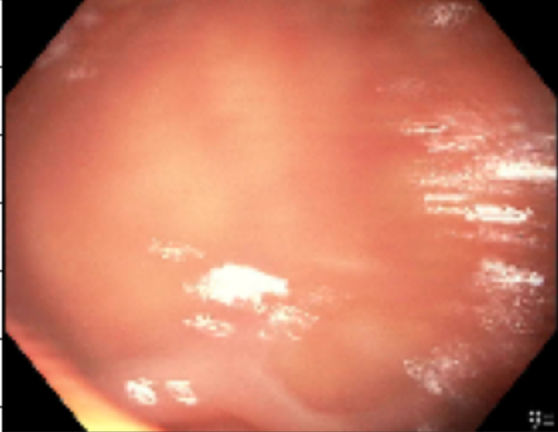
\includegraphics[width=\linewidth]{Materials/Discussion/idx_1_frame_550}
		\caption{Example of motion blur and glare (inflamed).}
	\end{subfigure}
	\hspace{0.5cm}
	\begin{subfigure}{0.4\linewidth}
		\centering
		
\includegraphics[width=\linewidth]{Materials/Discussion/idx_1_frame_1410}
		\caption{Example of all red frame (healthy).}
	\end{subfigure}
	\\
	\begin{subfigure}{0.4\linewidth}
		\centering
		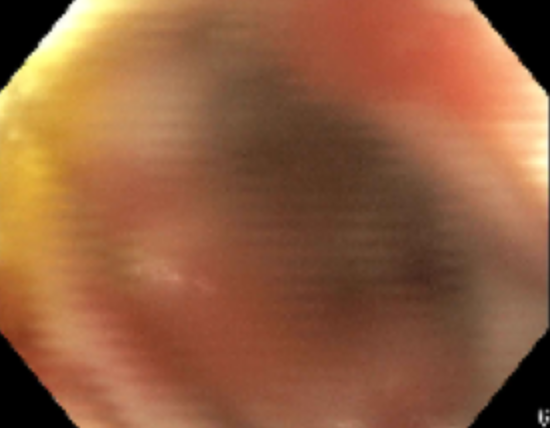
\includegraphics[width=\linewidth]{Materials/Discussion/idx_4_frame_750}
		\caption{Example of blurred frame (inflamed).\newline}
	\end{subfigure}
	\hspace{0.5cm}
	\begin{subfigure}{0.4\linewidth}
		\centering
		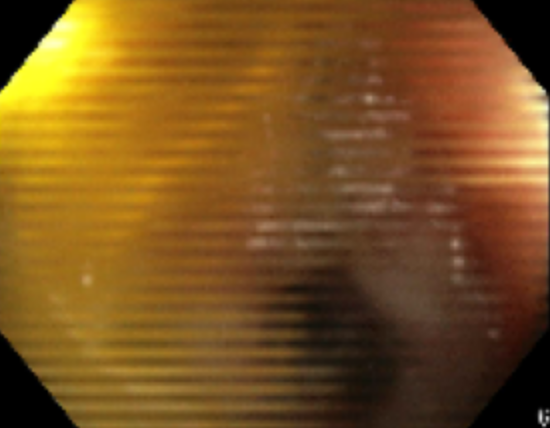
\includegraphics[width=\linewidth]{Materials/Discussion/idx_4_frame_840}
		\caption{Example of a large part of a frame changing colour to yellow (inflamed).}
	\end{subfigure}
	\caption{Examples of noisy frames in the endoscopy videos.}
	\label{noisyFrames}
\end{figure}

One could remove all of these frames from the training data, making it a lot easier for the model to find the needed features in the images to detect inflammation, however, when it is then presented with a video 'from the real world', it would likely not be able to generalize due to unseen noise.

To evaluate the performance of model \textit{Idx\_2\_3\_4\_5\_6\_skip\_20}, we take a look at its $65\%$ validation accuracy and at its predictions in \autoref{idx23}, \autoref{idx24} and \autoref{idx28}. Its accuracy is by itself not impressive, and especially not when taking into consideration about $72\%$ of the validation video are inflamed frames. Looking at its predictions, the model overly predicts inflammation, which leads to a conservative model which has a hard time predicting correctly on videos which are balanced or biased towards healthy frames. On the other hand, the model seems to perform decent on videos biased towards inflamed frames, where it most often finds some correct healthy frames. Although we should not expect perfect segmentation due to the noisy nature of the videos, we conclude none of the models are performing optimally, and model \textit{Idx\_2\_3\_4\_5\_6\_skip\_20} to a small degree produces usable results, however, they are not of a quality where they can contribute with any meaningful information to a doctor.

\subsection{Separation point predictions}
A general tendency for the Random Walker post-processing was to predict the separation point at the location of the last uncertainty in predictions. That is, the rightmost part of the segmentation where there would be either volatile predictions or elevated probability of predicting healthy. Because the Random Walker has a hard time crossing points or frames where the model predictions are dissimilar, this is somewhat expected, but due to the random noise in the videos previously discussed, this makes this approach conservative and not very robust. This was also verified as on average, the Random Walker approach would predict a separation point $51.85\%$ of the total number of frames in a video away from the true separation point. For the results produced by model \textit{Idx\_2\_3\_4\_5\_6\_skip\_20} this approach is thus not usable to predict the separation points.\\
Had we had more accurate predictions, the results would likely have been better, however, due to the noisy nature of the videos, and how the Random Walker would likely get 'stuck' on the noise, it is still questionable if this approach can produce meaningful results.

The scoring heuristic works by finding dissimilarities between the prediction probabilities of two consecutive frames. If the there is a high probability both frames belong to the same class, the score is high, whereas, if there is a high probability they belong to different classes, the score is low. Thus, this approach should be good at finding the transitions between frames where the model is insecure or predicts on noisy data. This is also generally what we see, and often one of the candidate points are near the true separation point, however, it is rare this candidate point holds the actual lowest score. As it on average would predict a separation point $51.87\%$ of the total number of frames in a video away from the true separation point, its 'believed separation point' is not usable to predict the separation points.\\
Providing candidate points could be useful for a doctor to do a quick evaluation based on the predicted segmentation and the candidate points. This could save the doctor time by not having to look the whole video through. But, as it is hard, if not impossible, to tell if any of the candidate points actually resembles the true separation point, only having the predicted segmentation available, the fact one of the candidate points often (but not always) is accurate is not of much help in practice.

\subsection{Treatment predictions}
While most treatment annotations are clear, some videos have been annotated with treatment 'x or y'. These cases are indices $7$ and $8$ which have been annotated as class $2$ or $3$, index 14 annotated class $2$ or $4$, index 28 annotated class $0$ or $1$ and indices 34 and 35 annotated class $1$ or $2$. In all these cases, the largest class number has been chosen as the true class, however, this might add or subtract a few percentages of accuracy depending on how the true classes are chosen.

In \autoref{treatmentTable} we saw the 1D ResNet model could achieve an accuracy of $40\%$, which is good considering random predictions would have yielded $20\%$ accuracy. However, if these predictions were to be used by a doctor, as for instance a second opinion, $40\%$ is rather low and would be too unreliable. We also see the model only predicting classes $0$ and $2$, which would indicate the model does not generalize too well.\\
Looking at \autoref{rocpreds} we see class $0$ and class $1$ having an area under the curve above $0.5$ which indicates the models have some measure of class separability whereas for classes $2$ and $3$ we see the scores being very close to $0.5$. Looking at class $4$, we have a score of $0.33$ which would indicate it is quite hard to predict correctly. When we look at class $3$ and $4$, we need to remember only 2 and 1 examples exists in the data, and thus the model will naturally have a hard time predicting these classes. If we look at the micro average, we see a score of $0.68$, which would indicate we can expect a model to have some measure of class separability when trained on this data, which we already have seen was the case. However, looking at the macro average which takes the class imbalance into consideration, we should not expect any meaningful results. This might, however, be skewed as class $3$ and $4$ have this few examples.

In \autoref{treatmentTableWithTrue} we added the true segmentations during training, and the accuracy increased to $48\%$. However, the model still only predicts class $0$ and $2$, indicating it overfits the training data. Looking at \autoref{rocpredsandtrue} we see the scores for class $0$ and $1$ almost swap, and the rest of the classes and the macro average staying very similar to what we had without adding the true segmentations. The micro average falls slightly, but still is at a level where some notion of class separability would be expected. The micro average falling, and yet the multi class classifier achieving a higher accuracy could be caused by the model predictions being closer to each other, i.e. the model is not as confident in its choice of class, but still ends up choosing the correct class.

Overall it would seem more tuning could have been done to achieve better results. Although nearing $50\%$ accuracy on a $5$ class classification problem seems decent, the ROC curves are not very confident, and even the highest scores being rather mediocre. Again training for more epochs with an accordingly lower learning rate could be a possible improvement. The indications of overfitting in both results would also point towards more regularization would be needed. Adding dropout to force the models to learn a wider array of features in the data could be one choice. As we are seeing the model is capable of solving the problem to some extent, a change of model architecture is most likely not needed to raise the performance.

\subsection{U-Net for video segmentation}
Opposite to ResNet, that would make its predictions on each individual image without considering the images before and after it, the U-Net models were trained on the segmentations, and because U-Net works on several levels of abstractions it would be expected to capture the 'structure' of the segmentations, i.e. how the true segmentations are blocks of first inflamed frames and then healthy frames. This structure is to a large degree missing from the initial 2D ResNet predictions, and thus the hope with the results of using the U-Net, was to bring this structure into the predictions.\\
Looking at \autoref{unetres1} and \autoref{unetres2} we see the U-Net overly predict healthy frames, which probably is a reaction to the ResNet overly predicting inflammation. The structure we were seeking, is also only brought back to a limited extent. Because the U-Net predictions overrule the correctly predicted frames from the ResNet, it seems the problem with the original predictions have just shifted from being overly many inflamed predictions to overly many healthy predictions. 

\subsection{U-Net predictions for treatment prediction}
Although the predictions of the U-Net models did not seem to make the results much more usable than the original 2D ResNet results, we see a big difference in how the treatments are predicted. In \autoref{unetPredsTreatmentTable} we now see predictions of class 0, 1 and 2. Because of the low number of examples of class 3 and 4 treatments, it is not surprising we do not see these classes predicted. We now have an accuracy of $52\%$ which, taking into consideration we have 5 classes, is decent. However, it is still not high enough to, for instance, act as a second opinion for a doctor. Looking at \autoref{rocunetpreds} we now see a drastic drop in the area under the ROC curves. We now only have class 4 not being near a score of $0.5$. Given how the 'one-vs-rest' classifiers struggle, the high accuracy could be caused by the multi class classifier not being very confident and having almost equal probabilities for each class, but the correct class coming out on top for the most part.

In \autoref{unetPredsTrueTreatmentTable} the true segmentations were added to the training. We still see the model predicting class 0, 1 and 2, however, we now see the accuracy drop to $20\%$, indicating random guesses were made. Looking at \autoref{rocunetpredstrue} we however see class 0 having a score of $0.66$, suggesting these predictions were not entirely random. The rest of the classes do struggle however. It is likely adding the true segmentations simply confused the model during training, as the features found in the predicted segmentations did not match the features found for the true segmentations. Also, the drop in accuracy could stem from the multi class classifier not being confident in its predictions, giving almost equal probabilities to each class, but this time the correct classes would not come out on top.

















